\documentclass[12pt]{article}

\usepackage{ee143report}
\usepackage{verbatim}
\usepackage{graphicx, float}
\usepackage{enumerate}
\usepackage{amsmath}
\usepackage{bookmark}
\usepackage{pdflscape}
\usepackage{multirow}
\usepackage{hyperref}

\DeclareMathOperator{\V}{V}
\DeclareMathOperator{\A}{A}
\DeclareMathOperator{\F}{F}
\DeclareMathOperator{\mA}{mA}
\DeclareMathOperator{\mW}{mW}
\DeclareMathOperator\bit{bit}
\DeclareMathOperator\byte{byte}
\DeclareMathOperator\word{word}

\author{Astrid Yu}
\title{Voltage Division and Loading Effects}
\expNum{5}
\titlegraphic{
    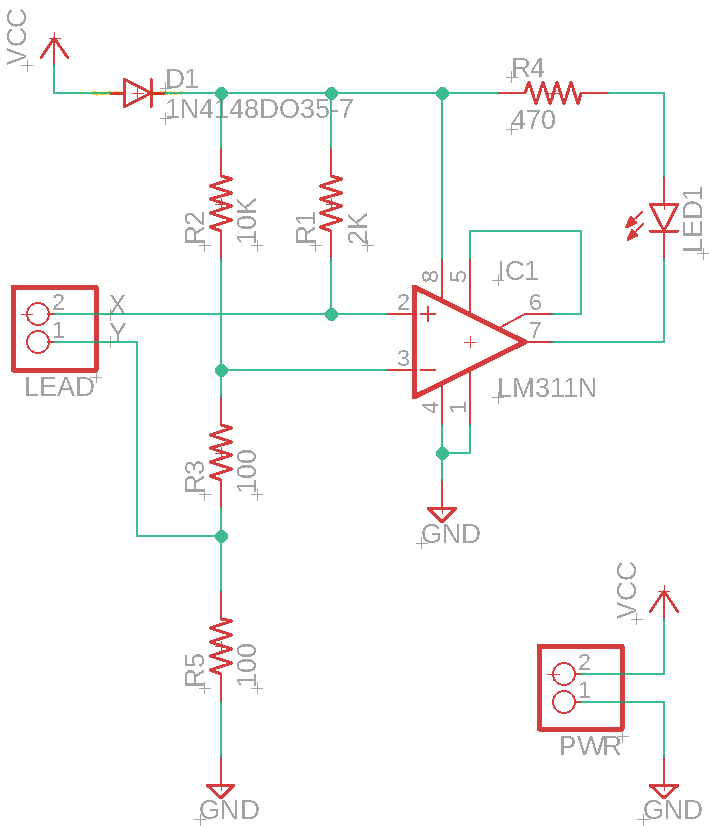
\includegraphics[width=0.5\linewidth]{sch.png}
}

\begin{document}
\maketitle

\section*{Introduction}

The purpose of this experiment is to investigate loading effects and ways 
to mitigate them. This will be aided with LTSpice. Additionally, an 
analog-to-digital converter (ADC) will be used in conjunction with a 
thermistor for the purpose of temperature measurement. 

\section*{Analysis}

\begin{figure}[]
    \centering
    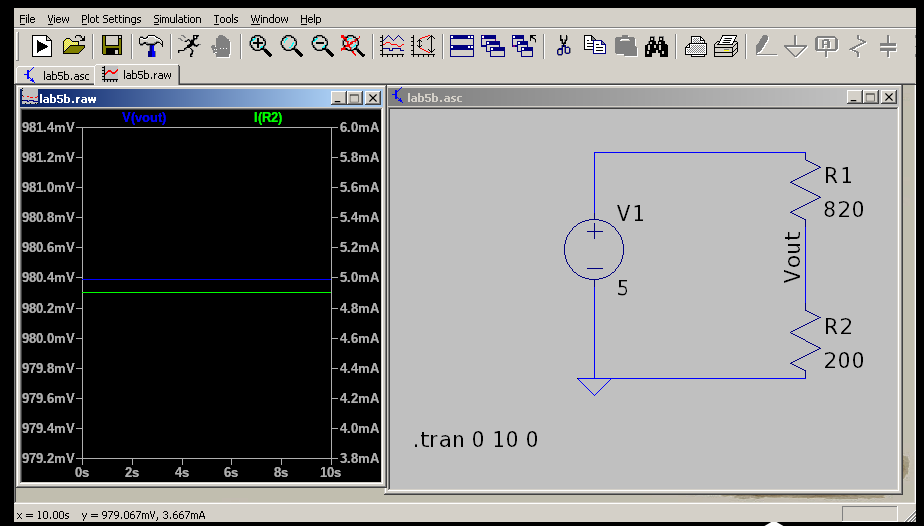
\includegraphics[width=0.9\linewidth]{lab2.png}
    \caption{The voltage divider circuit, simulated in LTSpice.}
    \label{fig:simcircuit}
\end{figure}

\subsection*{1. Voltage Division: Level Shifting}

\begin{enumerate}[a.]
    \item The circuit shown in Figure \ref{fig:simcircuit} was constructed on a breadboard using an
        Arduino as the power source and $2\times 100 \Omega$ resistors in series to act as R2, which
        is a single $200\Omega$ resistor. The voltage across and current through R2 were measured 
        and recorded in Table \ref{tbl:measresults}.
    \item A buzzer was connected across R2, and measurements and observations were recorded in 
        Table \ref{tbl:measresults}.

        \textbf{Is the buzzer getting the intended voltage and current?}

        No.

        \textbf{Is the buzzer making a sound? What happened?}
        
        The buzzer was not making much sound, just somewhat vibrating, because there was not enough 
        power delivered to it to make sound.

    \item The buzzer was replaced with a motor, and measurements and observations were recorded in 
        Table \ref{tbl:measresults}. 

        \textbf{Is the motor getting the intended voltage and current?}

        No.

        \textbf{What happened?}

        There was insufficient current supplied to the motor, so it could not overcome friction. 

\end{enumerate}

\subsection*{2. Voltage Follower and FET as a Switch}

\begin{enumerate}[a.]
    \item The voltage follower circuit depicted in Figure \ref{fig:vfollow} was constructed. 
    \begin{figure}[H]
        \centering
        \includegraphics[width=\linewidth]{vfollow.png}
        \caption{Voltage follower circuit.}
        \label{fig:vfollow}
    \end{figure}
        
    \item A buzzer was connected in the load position. The voltage across and current 
        through were recorded in Table \ref{tbl:measresults}.
    \item The buzzer was replaced with a motor, and the same measurements were made and 
        recorded in Table \ref{tbl:measresults}.
    \item The FET circuit depicted in Figure \ref{fig:fet} was constructed. A motor was placed 
        in the load position, and its voltage across and current through were recorded in 
        \ref{tbl:measresults}. The motor was replaced with a buzzer, and the same 
        measurements were recorded.
        \begin{figure}[H]
            \centering
            \includegraphics[width=0.3\linewidth]{fet.png}
            \caption{FET circuit.}
            \label{fig:fet}
        \end{figure}
        
\end{enumerate}

\begin{landscape}
    \begin{table}
        \centering
        \caption{Summarized Data from Sections 1 and 2.}
        \begin{tabular}{| c | c || c | r | r | p{5.5cm} |}
            \hline
            \textbf{Configuration} & \textbf{Load} & \textbf{Measured Device} & \textbf{Voltage (V)} & \textbf{Current (mA)} & \textbf{Observations}  \\
            \hline
            Simulation & none & R2 & 0.9804 & 4.9 & --- \\
    
            \hline
            \multirow{7}{*}{Simple Divider} & none & R2 & 0.990 & 4.98 & --- \\
            \cline{2-6}
    
            & Buzzer & Buzzer & 0.913 & 0.48 & Very weak buzzing. Loudness depended on how it was placed or held. \\
            \cline{2-6}
    
            & Motor & Motor & 0.00134 & 6.05 & No spinning. When manually spun, less resistance felt one direction than other direction. \\
            \cline{2-6}
            \hline
    
            \multirow{3}{*}{Voltage Follower} & Buzzer & Buzzer & 0.988 & 4.92 & Very loud. \\
            \cline{2-6}
            & Motor & Motor & 0.00733 & 34.8 & No spinning, but even less resistance when manually spun. \\
            \hline
    
            \multirow{3}{*}{FET} & Buzzer & Buzzer & 4.90 & 44.3 & Extremely loud. \\
            \cline{2-6}
            & Motor & Motor & 0.017 & 8.31 & Spins. Measured after the motor reached equilibrium speed. \\
            \hline
        \end{tabular}

        \label{tbl:measresults}
    \end{table}        
\end{landscape}

\subsection*{3. Voltage Division: Reading Resistive Sensors}

\begin{enumerate}[a.]
    \item An Arduino was connected to the computer, and Arduino IDE was opened.
    \item The correct board and port were selected. 
    \item The 3.3V pin was connected to the A0 pin.
    \item The AnalogReadSerial example was uploaded, and values typically ranging between 689
    and 691 were observed, as seen in Figure \ref{fig:a03}.
    \begin{figure}[H]
        \centering
        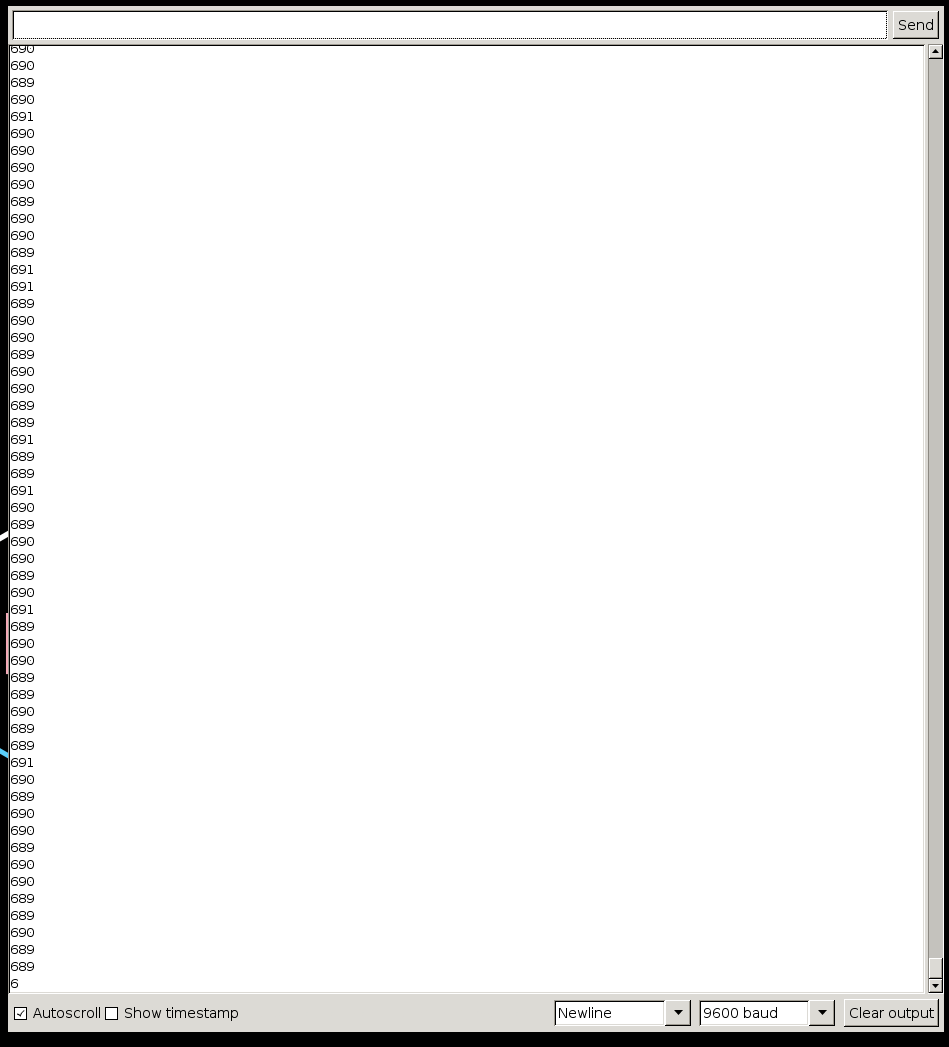
\includegraphics[width=0.5\linewidth]{sermon.png}
        \caption{Serial output when 3.3v was connected to A0.}
        \label{fig:a03}
    \end{figure}
        
    \item 5V was connected to the A0 pin, and 1023 only was observed as seen in Figure \ref{fig:a05}. 
        Next, GND was connected to the A0 pin, and 0 only was observed as seen in Fighre \ref{fig:a00}.
    
        \begin{figure}[H]
            \centering
            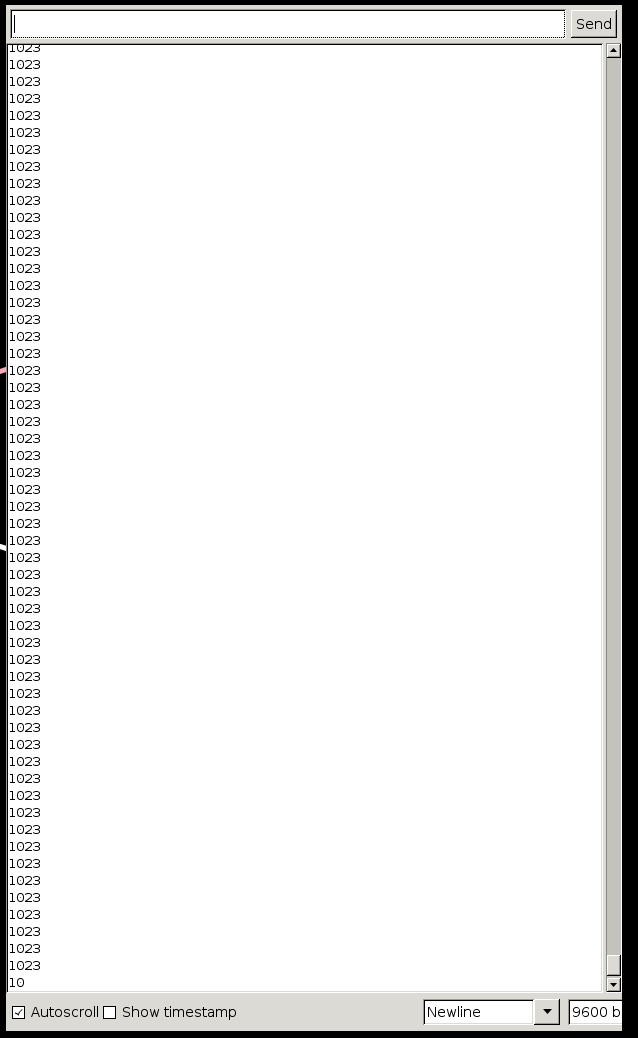
\includegraphics[width=0.4\linewidth]{5v.png}
            \caption{Serial output when 5v was connected to A0.}
            \label{fig:a05}
        \end{figure}
        
        \begin{figure}[H]
            \centering
            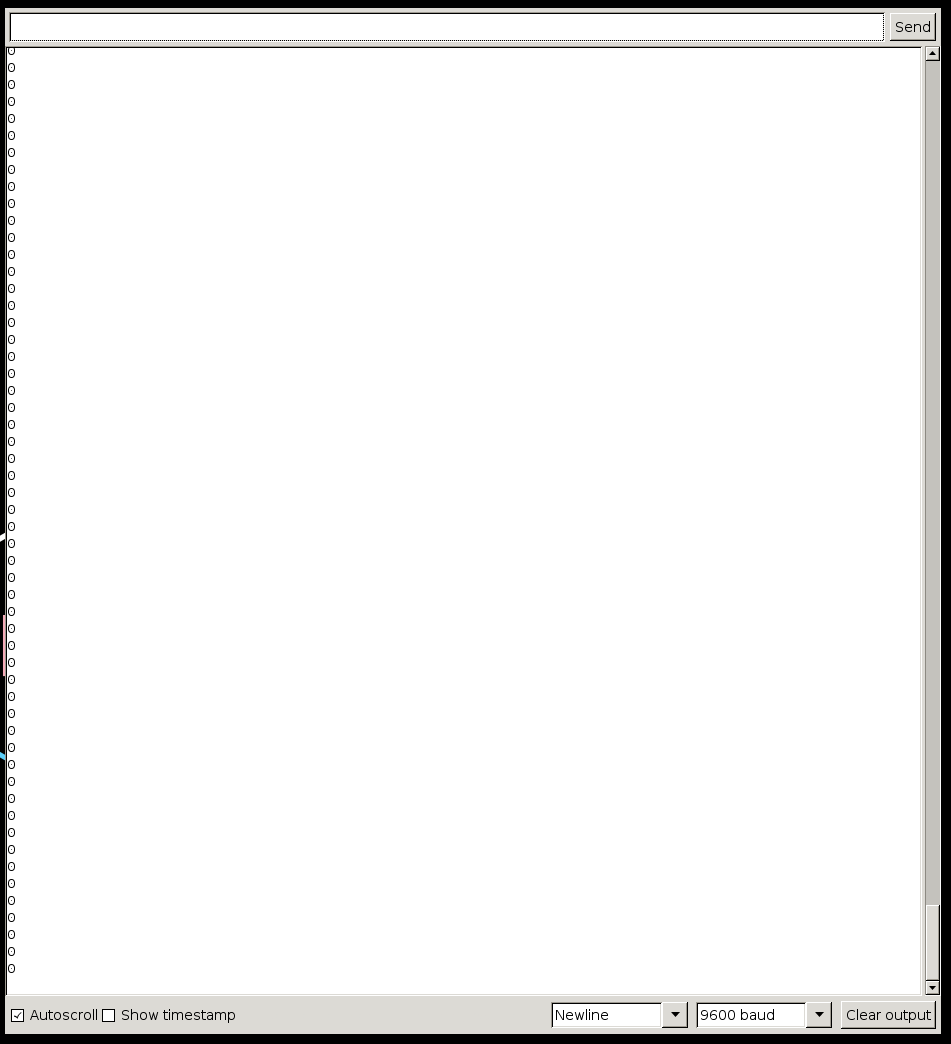
\includegraphics[width=0.5\linewidth]{sermon2.png}
            \caption{Serial output when GND was connected to A0.}
            \label{fig:a00}
        \end{figure}
        
        
    \item The circuit shown in Figure \ref{fig:sch} was constructed. 
    \item The AnalogReadSerial program was modified to print the temperature in Fahrenheit every 
    5 seconds using the equations as follows.

    Let $R$ be the resistance of the thermistor, $T$ be the temperature sensed by the 
    thermistor, $V$ be the voltage measured by the on-board ADC, and $X$ be the 10-bit value 
    reported by the ADC. Their relationships are described by the following three equations, which
    were derived during the pre-lab:
    \begin{equation}
        V = \frac{5\V}{2^{10}}\cdot X
    \end{equation}
    \begin{equation}
        R = \frac{V \cdot 2k\Omega}{5\V - V}
    \end{equation}
    \begin{equation}
        T=(0.1056\frac{^\circ \F}{\Omega}) \cdot R -146.4 ^\circ\F
    \end{equation}

    They were combined on the Arduino to derive temperature from voltage divider output.

    \item Finally, the program was tested, first by heating up the thermistor as shown in 
    Figure \ref{fig:warming}, and then by cooling it back down, as shown in Figure \ref{fig:cooling}.
    The serial output is displayed in Figure \ref{fig:tempser}, confirming that the program 
    and thermistor work.
\end{enumerate}

\begin{figure}[H]
    \centering
    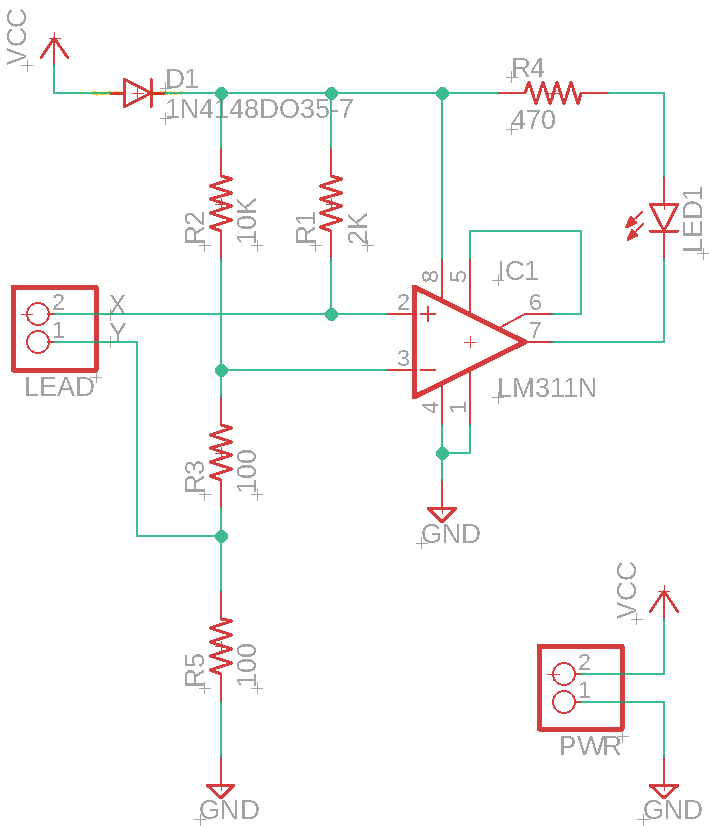
\includegraphics[width=\linewidth]{sch.png}
    \caption{Thermistor voltage divider circuit. Note that the R2, the PTC-SOD70 (positive thermal 
    coefficient resistor, SOD70 footprint) represents the KTY81-210.}
    \label{fig:sch}
\end{figure}

\begin{figure}[H]
    \centering
    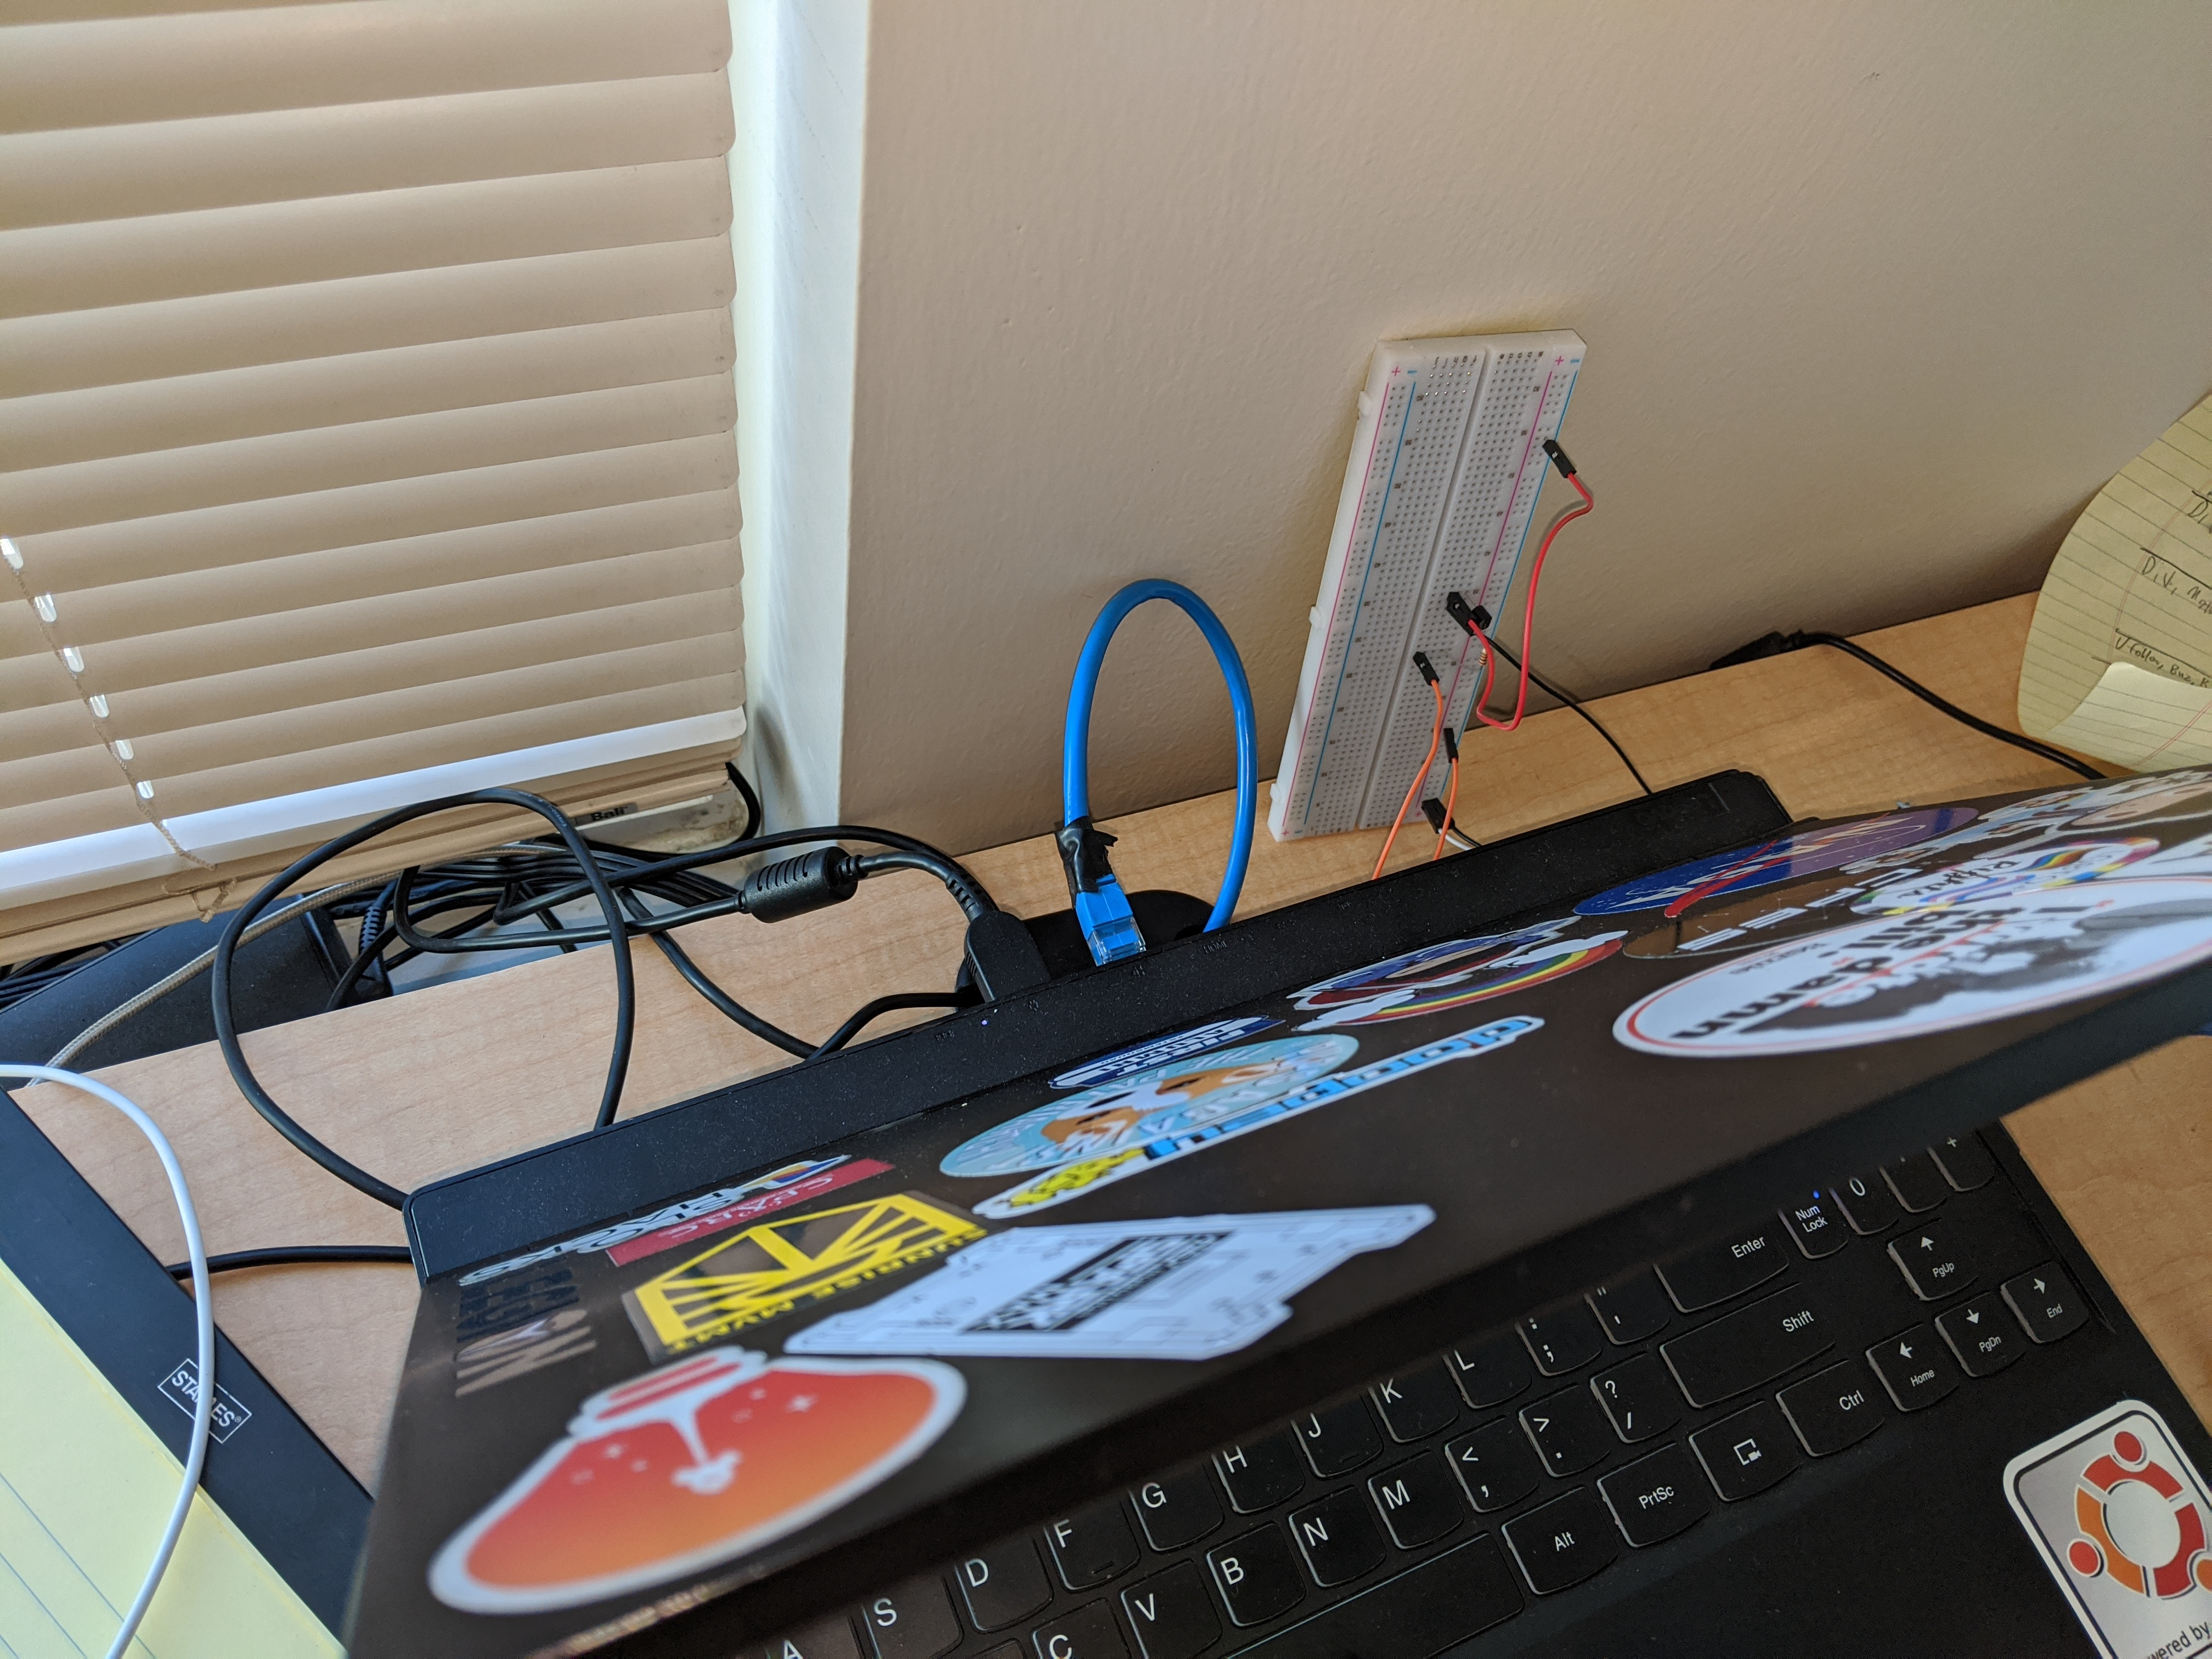
\includegraphics[width=0.7\linewidth]{warming.jpg}
    \caption{Thermistor warming setup. The heat from the laptop (generated while operating a modern 
    IDE) raises the temperature of the thermistor.}
    \label{fig:warming}
\end{figure}

\begin{figure}[H]
    \centering
    \includegraphics[width=0.7\linewidth]{cooling.jpg}
    \caption{Thermistor cooling setup. The breadboard was placed inside a bladeless
    fan to facilitate heat transfer out of the thermistor and into the air.}
    \label{fig:cooling}
\end{figure}

\begin{figure}[H]
    \centering
    \includegraphics[width=0.6\linewidth]{temp.png}
    \caption{Serial output from thermistor experiment, with timestamps turned on. The 
    red-highlighted section was during the warming phase, and the blue-highlighted section
    was from the cooling phase. Observe how the temperatures are increasing and decreasing 
    in their respective phases, indicating that the thermistor and program are working 
    as expected.}
    \label{fig:tempser}
\end{figure}

\section*{Discussion Questions}

\subsection*{Section 1}

\begin{enumerate}
    \item LTSpice is good for simulating circuits, but due to tolerance levels and such, 
        it will not be 100\% accurate. The approximate prediction
        error of the simulation can be calculated using the following equation:
        \begin{equation}
            \frac{(\text{predicted}) - (\text{measured})}{(\text{measured})} \cdot 100 \%
        \end{equation}

        Plugging in the values from Table \ref{tbl:measresults}, the voltage error was
        \begin{equation}
            \frac{0.9804\V - 0.990\V}{0.990\V} = -0.96\%
        \end{equation}

        and the current error was
        \begin{equation}
            \frac{4.9\mA - 4.98\mA}{4.98\mA} = -2\%
        \end{equation}

        The resistors used in this experiment had 5\% tolerance, so the error here is well
        within expected bounds, and LTSpice was fairly accurate.

        However, LTSpice does have a Monte Carlo simulation function (not used in this
        experiment) that can be used to help it account for these errors, if the requirements
        are very strict and the device being powered is very sensitive to small changes.
    \item The circuit did provide a fairly good voltage of 0.913V across the buzzer, but 
        it did not provide enough current through the buzzer (only 0.48mA).
        \footnote{See table \ref{tbl:measresults}} This is because a relatively large resistance 
        was placed in front of the buzzer ($820\Omega$), severely limiting the 
        maximum current that can pass through.
\end{enumerate}
\subsection*{Section 2}
\begin{enumerate}
    \item A field-effect transistor, or FET, can be used as an alternative to voltage 
        followers for reducing loading effects. 
    \item A voltage follower can prevent loading for applications which require a stable 
        voltage, but it cannot prevent loading for those that require extra current.
\end{enumerate}

\subsection*{Section 3}

The code used to measure the resistance of the thermistor and calculate the 
temperature is shown here.

\begin{verbatim}
void setup() {
  Serial.begin(9600);
}

void loop() {
  int sensorValue = analogRead(A0);
  float volts = 5.0 * sensorValue / 1024.0;
  float resistance = volts * 2000 / (5 - volts);
  float temp = 0.1056 * resistance - 146.4;

  Serial.println(temp);
  delay(5000); 
}

\end{verbatim}

\section*{Conclusion}

In this experiment, loading effects were measured, quantified, and prevented
using special components that amplify and stabilize precise-voltage, low-current 
signals. A voltage follower was found to be useful for low-current applications, 
such as a buzzer, and a FET was found to be useful for high-current applications,
such as a motor. 

\end{document}
